% Options for packages loaded elsewhere
\PassOptionsToPackage{unicode}{hyperref}
\PassOptionsToPackage{hyphens}{url}
%
\documentclass[
  ignorenonframetext,
]{beamer}
\usepackage{pgfpages}
\setbeamertemplate{caption}[numbered]
\setbeamertemplate{caption label separator}{: }
\setbeamercolor{caption name}{fg=normal text.fg}
\beamertemplatenavigationsymbolsempty
% Prevent slide breaks in the middle of a paragraph
\widowpenalties 1 10000
\raggedbottom
\setbeamertemplate{part page}{
  \centering
  \begin{beamercolorbox}[sep=16pt,center]{part title}
    \usebeamerfont{part title}\insertpart\par
  \end{beamercolorbox}
}
\setbeamertemplate{section page}{
  \centering
  \begin{beamercolorbox}[sep=12pt,center]{part title}
    \usebeamerfont{section title}\insertsection\par
  \end{beamercolorbox}
}
\setbeamertemplate{subsection page}{
  \centering
  \begin{beamercolorbox}[sep=8pt,center]{part title}
    \usebeamerfont{subsection title}\insertsubsection\par
  \end{beamercolorbox}
}
\AtBeginPart{
  \frame{\partpage}
}
\AtBeginSection{
  \ifbibliography
  \else
    \frame{\sectionpage}
  \fi
}
\AtBeginSubsection{
  \frame{\subsectionpage}
}
\usepackage{amsmath,amssymb}
\usepackage{iftex}
\ifPDFTeX
  \usepackage[T1]{fontenc}
  \usepackage[utf8]{inputenc}
  \usepackage{textcomp} % provide euro and other symbols
\else % if luatex or xetex
  \usepackage{unicode-math} % this also loads fontspec
  \defaultfontfeatures{Scale=MatchLowercase}
  \defaultfontfeatures[\rmfamily]{Ligatures=TeX,Scale=1}
\fi
\usepackage{lmodern}
\usetheme[]{CambridgeUS}
\usecolortheme{seagull}
\usefonttheme{professionalfonts}
\ifPDFTeX\else
  % xetex/luatex font selection
\fi
% Use upquote if available, for straight quotes in verbatim environments
\IfFileExists{upquote.sty}{\usepackage{upquote}}{}
\IfFileExists{microtype.sty}{% use microtype if available
  \usepackage[]{microtype}
  \UseMicrotypeSet[protrusion]{basicmath} % disable protrusion for tt fonts
}{}
\makeatletter
\@ifundefined{KOMAClassName}{% if non-KOMA class
  \IfFileExists{parskip.sty}{%
    \usepackage{parskip}
  }{% else
    \setlength{\parindent}{0pt}
    \setlength{\parskip}{6pt plus 2pt minus 1pt}}
}{% if KOMA class
  \KOMAoptions{parskip=half}}
\makeatother
\usepackage{xcolor}
\newif\ifbibliography
\usepackage{color}
\usepackage{fancyvrb}
\newcommand{\VerbBar}{|}
\newcommand{\VERB}{\Verb[commandchars=\\\{\}]}
\DefineVerbatimEnvironment{Highlighting}{Verbatim}{commandchars=\\\{\}}
% Add ',fontsize=\small' for more characters per line
\usepackage{framed}
\definecolor{shadecolor}{RGB}{248,248,248}
\newenvironment{Shaded}{\begin{snugshade}}{\end{snugshade}}
\newcommand{\AlertTok}[1]{\textcolor[rgb]{0.94,0.16,0.16}{#1}}
\newcommand{\AnnotationTok}[1]{\textcolor[rgb]{0.56,0.35,0.01}{\textbf{\textit{#1}}}}
\newcommand{\AttributeTok}[1]{\textcolor[rgb]{0.13,0.29,0.53}{#1}}
\newcommand{\BaseNTok}[1]{\textcolor[rgb]{0.00,0.00,0.81}{#1}}
\newcommand{\BuiltInTok}[1]{#1}
\newcommand{\CharTok}[1]{\textcolor[rgb]{0.31,0.60,0.02}{#1}}
\newcommand{\CommentTok}[1]{\textcolor[rgb]{0.56,0.35,0.01}{\textit{#1}}}
\newcommand{\CommentVarTok}[1]{\textcolor[rgb]{0.56,0.35,0.01}{\textbf{\textit{#1}}}}
\newcommand{\ConstantTok}[1]{\textcolor[rgb]{0.56,0.35,0.01}{#1}}
\newcommand{\ControlFlowTok}[1]{\textcolor[rgb]{0.13,0.29,0.53}{\textbf{#1}}}
\newcommand{\DataTypeTok}[1]{\textcolor[rgb]{0.13,0.29,0.53}{#1}}
\newcommand{\DecValTok}[1]{\textcolor[rgb]{0.00,0.00,0.81}{#1}}
\newcommand{\DocumentationTok}[1]{\textcolor[rgb]{0.56,0.35,0.01}{\textbf{\textit{#1}}}}
\newcommand{\ErrorTok}[1]{\textcolor[rgb]{0.64,0.00,0.00}{\textbf{#1}}}
\newcommand{\ExtensionTok}[1]{#1}
\newcommand{\FloatTok}[1]{\textcolor[rgb]{0.00,0.00,0.81}{#1}}
\newcommand{\FunctionTok}[1]{\textcolor[rgb]{0.13,0.29,0.53}{\textbf{#1}}}
\newcommand{\ImportTok}[1]{#1}
\newcommand{\InformationTok}[1]{\textcolor[rgb]{0.56,0.35,0.01}{\textbf{\textit{#1}}}}
\newcommand{\KeywordTok}[1]{\textcolor[rgb]{0.13,0.29,0.53}{\textbf{#1}}}
\newcommand{\NormalTok}[1]{#1}
\newcommand{\OperatorTok}[1]{\textcolor[rgb]{0.81,0.36,0.00}{\textbf{#1}}}
\newcommand{\OtherTok}[1]{\textcolor[rgb]{0.56,0.35,0.01}{#1}}
\newcommand{\PreprocessorTok}[1]{\textcolor[rgb]{0.56,0.35,0.01}{\textit{#1}}}
\newcommand{\RegionMarkerTok}[1]{#1}
\newcommand{\SpecialCharTok}[1]{\textcolor[rgb]{0.81,0.36,0.00}{\textbf{#1}}}
\newcommand{\SpecialStringTok}[1]{\textcolor[rgb]{0.31,0.60,0.02}{#1}}
\newcommand{\StringTok}[1]{\textcolor[rgb]{0.31,0.60,0.02}{#1}}
\newcommand{\VariableTok}[1]{\textcolor[rgb]{0.00,0.00,0.00}{#1}}
\newcommand{\VerbatimStringTok}[1]{\textcolor[rgb]{0.31,0.60,0.02}{#1}}
\newcommand{\WarningTok}[1]{\textcolor[rgb]{0.56,0.35,0.01}{\textbf{\textit{#1}}}}
\setlength{\emergencystretch}{3em} % prevent overfull lines
\providecommand{\tightlist}{%
  \setlength{\itemsep}{0pt}\setlength{\parskip}{0pt}}
\setcounter{secnumdepth}{-\maxdimen} % remove section numbering
\usepackage{placeins}
\usepackage{color}
\usepackage{bm}
\usepackage{amsmath}
\usepackage{algorithm}
\usepackage[]{algpseudocode}
\usepackage{tabularx}
\usepackage{multirow}
\usepackage[most]{tcolorbox}
\usepackage{tikz}
\usepackage{lipsum}
\usepackage{mathtools}
\usepackage{actuarialangle}
\usepackage{multirow, longtable, array, dcolumn}
\usepackage{tabu}
\newcommand{\sdt}{\bullet}
\newcommand{\tss}{\textsuperscript}
\newcommand{\morearraysp}{\setlength{\arraycolsep}{2mm}}
\newcommand{\smarraysp}{\setlength{\arraycolsep}{1mm}}
\newcommand{\oldarraysp}{\setlength{\arraycolsep}{1.5pt}}
\newcommand{\matrixstretch}{\setlength{\extrarowheight}{4pt}}
\newcommand{\matrixnostretch}{\setlength{\extrarowheight}{0pt}}
\newcommand{\gil}[1]{\textrm{\gilfont{#1}}\normalfont }
\newfont{\gilfont}{msbm10 scaled 1000}
\newcommand{\DOT}{\usebox{\biggercirc}}
\newcommand{\pv}{\wp\text{-value}}
\ifLuaTeX
  \usepackage{selnolig}  % disable illegal ligatures
\fi
\IfFileExists{bookmark.sty}{\usepackage{bookmark}}{\usepackage{hyperref}}
\IfFileExists{xurl.sty}{\usepackage{xurl}}{} % add URL line breaks if available
\urlstyle{same}
\hypersetup{
  pdftitle={MAT 3850 : Week 2},
  pdfauthor={Spring 2024},
  hidelinks,
  pdfcreator={LaTeX via pandoc}}

\title{MAT 3850 : Week 2}
\author{Spring 2024}
\date{}
\institute{Appalachian State University}

\begin{document}
\frame{\titlepage}

\hypertarget{outline-for-the-week}{%
\section{Outline for the week}\label{outline-for-the-week}}

\begin{frame}{By the end of the week:}
\protect\hypertarget{by-the-end-of-the-week}{}
\begin{itemize}
\tightlist
\item
  Control Structures in R
\item
  \href{https://quarto.org/}{Quarto}
\item
  Data Visualization
\end{itemize}
\end{frame}

\hypertarget{control-structures-in-r}{%
\section{Control Structures in R}\label{control-structures-in-r}}

\begin{frame}[fragile]{Control Structures in R}
\protect\hypertarget{control-structures-in-r-1}{}
\texttt{R} executes statements/commands sequentially. If you want to
control the flow of statement execution, you need to use \textbf{control
structures}.

\begin{itemize}
\item
  The basic component of most control structures is the
  \textbf{conditional statement}.
\item
  A conditional statement is an \texttt{R} statement that is evaluated
  as either TRUE or FALSE. They use relational operators such as

  \begin{itemize}
  \item
    \texttt{==} for testing equality of R objects,
  \item
    \texttt{!=} for testing if two \texttt{R} objects are not equal,
    \textless,\textgreater{} ,\textless= and \textgreater=.
  \end{itemize}
\end{itemize}

As an example, look at the following R commands:
\end{frame}

\begin{frame}[fragile]{Conditional Statement}
\protect\hypertarget{conditional-statement}{}
\small

\begin{Shaded}
\begin{Highlighting}[]
\NormalTok{x }\OtherTok{\textless{}{-}} \FunctionTok{c}\NormalTok{(}\DecValTok{1}\NormalTok{, }\DecValTok{2}\NormalTok{, }\DecValTok{3}\NormalTok{)  }\CommentTok{\# creates a vector named x}
\NormalTok{y }\OtherTok{\textless{}{-}} \FunctionTok{c}\NormalTok{(}\DecValTok{1}\NormalTok{, }\DecValTok{2}\NormalTok{, }\DecValTok{4}\NormalTok{)}
\NormalTok{x }\SpecialCharTok{==}\NormalTok{ y}
\end{Highlighting}
\end{Shaded}

\begin{verbatim}
[1]  TRUE  TRUE FALSE
\end{verbatim}

\normalsize

\begin{itemize}
\tightlist
\item
  The result of executing the last command is a vector containing the
  logical values TRUE, TRUE and FALSE since the only elements of the
  vectors \texttt{x} and \texttt{y} that are not equal are the 3rd
  elements.
\end{itemize}

Similarly,

\small

\begin{Shaded}
\begin{Highlighting}[]
\NormalTok{x }\SpecialCharTok{!=}\NormalTok{ y}
\end{Highlighting}
\end{Shaded}

\begin{verbatim}
[1] FALSE FALSE  TRUE
\end{verbatim}

\normalsize
\end{frame}

\begin{frame}[fragile]{Conditional Statement and Logical Operators}
\protect\hypertarget{conditional-statement-and-logical-operators}{}
\begin{itemize}
\item
  Conditional statements can be combined using logical operators
  \texttt{\&}, \texttt{\textbar{}} and \texttt{!}.

  \begin{itemize}
  \tightlist
  \item
    The operator \texttt{\&} means AND.
  \item
    The operator \texttt{\textbar{}} means OR
  \item
    and the operator \texttt{!} means NOT.
  \end{itemize}
\end{itemize}

As an example of the use of \texttt{\&}, the following will yield TRUE
since both conditions are TRUE.

\small

\begin{Shaded}
\begin{Highlighting}[]
\NormalTok{(x[}\DecValTok{1}\NormalTok{] }\SpecialCharTok{==}\NormalTok{ y[}\DecValTok{1}\NormalTok{]) }\SpecialCharTok{\&}\NormalTok{ (x[}\DecValTok{2}\NormalTok{] }\SpecialCharTok{==}\NormalTok{ y[}\DecValTok{2}\NormalTok{])}
\end{Highlighting}
\end{Shaded}

\begin{verbatim}
[1] TRUE
\end{verbatim}

\normalsize

On the other hand, \small

\begin{Shaded}
\begin{Highlighting}[]
\NormalTok{(x[}\DecValTok{1}\NormalTok{] }\SpecialCharTok{==}\NormalTok{ y[}\DecValTok{1}\NormalTok{]) }\SpecialCharTok{\&}\NormalTok{ (x[}\DecValTok{3}\NormalTok{] }\SpecialCharTok{==}\NormalTok{ y[}\DecValTok{3}\NormalTok{])}
\end{Highlighting}
\end{Shaded}

\begin{verbatim}
[1] FALSE
\end{verbatim}

\normalsize
\end{frame}

\begin{frame}[fragile]{Conditional Statement and Logical Operators}
\protect\hypertarget{conditional-statement-and-logical-operators-1}{}
However, the following will yield TRUE since at least one condition is
TRUE. That is, the \texttt{\textbar{}} operator will yield TRUE if at
least one of the conditions is TRUE.

\small

\begin{Shaded}
\begin{Highlighting}[]
\NormalTok{(x[}\DecValTok{1}\NormalTok{] }\SpecialCharTok{==}\NormalTok{ y[}\DecValTok{1}\NormalTok{]) }\SpecialCharTok{|}\NormalTok{ (x[}\DecValTok{3}\NormalTok{] }\SpecialCharTok{==}\NormalTok{ y[}\DecValTok{3}\NormalTok{])}
\end{Highlighting}
\end{Shaded}

\begin{verbatim}
[1] TRUE
\end{verbatim}

\normalsize

To negate the truth value of the above statement, use \texttt{!}:

\small

\begin{Shaded}
\begin{Highlighting}[]
\SpecialCharTok{!}\NormalTok{((x[}\DecValTok{1}\NormalTok{] }\SpecialCharTok{==}\NormalTok{ y[}\DecValTok{1}\NormalTok{]) }\SpecialCharTok{|}\NormalTok{ (x[}\DecValTok{3}\NormalTok{] }\SpecialCharTok{==}\NormalTok{ y[}\DecValTok{3}\NormalTok{]))}
\end{Highlighting}
\end{Shaded}

\begin{verbatim}
[1] FALSE
\end{verbatim}

\normalsize

Note the use of parentheses.
\end{frame}

\begin{frame}[fragile]{Conditional Statement and Logical Operators}
\protect\hypertarget{conditional-statement-and-logical-operators-2}{}
To see the effect of parentheses, let's remove the parentheses in the
previous statement. \small

\begin{Shaded}
\begin{Highlighting}[]
\SpecialCharTok{!}\NormalTok{(x[}\DecValTok{3}\NormalTok{] }\SpecialCharTok{==}\NormalTok{ y[}\DecValTok{3}\NormalTok{]) }\SpecialCharTok{|}\NormalTok{ (x[}\DecValTok{1}\NormalTok{]}\SpecialCharTok{==}\NormalTok{y[}\DecValTok{1}\NormalTok{])}
\end{Highlighting}
\end{Shaded}

\begin{verbatim}
[1] TRUE
\end{verbatim}

\normalsize

A control structure that uses conditional statement(s) is the \textbf{if
statement} and its variant \textbf{if else} and \textbf{if else if}.

\begin{itemize}
\tightlist
\item
  The if statement will perform an R command or a series of R commands
  only if the conditional statement is TRUE.
\end{itemize}

Lets see an example.
\end{frame}

\begin{frame}[fragile]{If Statement}
\protect\hypertarget{if-statement}{}
The following will display the value of the sum of the first two
elements of the vector \texttt{x} since the conditional statement is
TRUE.

\small

\begin{Shaded}
\begin{Highlighting}[]
\ControlFlowTok{if}\NormalTok{ (x[}\DecValTok{1}\NormalTok{] }\SpecialCharTok{==}\NormalTok{ y[}\DecValTok{1}\NormalTok{])\{}
\NormalTok{  sumx }\OtherTok{\textless{}{-}}\NormalTok{ x[}\DecValTok{1}\NormalTok{] }\SpecialCharTok{+}\NormalTok{ x[}\DecValTok{2}\NormalTok{]}
\NormalTok{  sumx}
\NormalTok{\}}
\end{Highlighting}
\end{Shaded}

\begin{verbatim}
[1] 3
\end{verbatim}

\normalsize

Similarly, the following code will not display anything since the
conditional statement is FALSE and hence R will not execute the R
statements within the square brackets.

\small

\begin{Shaded}
\begin{Highlighting}[]
\ControlFlowTok{if}\NormalTok{ (x[}\DecValTok{1}\NormalTok{] }\SpecialCharTok{!=}\NormalTok{ y[}\DecValTok{1}\NormalTok{])\{}
\NormalTok{  sumy }\OtherTok{\textless{}{-}}\NormalTok{ y[}\DecValTok{1}\NormalTok{] }\SpecialCharTok{+}\NormalTok{ y[}\DecValTok{2}\NormalTok{]}
\NormalTok{  sumy}
\NormalTok{\}}
\end{Highlighting}
\end{Shaded}

\normalsize
\end{frame}

\begin{frame}{If Statement}
\protect\hypertarget{if-statement-1}{}
Note that the syntax of an if statement is as follows

\begin{itemize}
\item
  if (conditional statement) \{R statements\}

  \begin{itemize}
  \tightlist
  \item
    brackets are optional if there is only one R statement
  \end{itemize}
\item
  If you want R to perform either a series of R statements

  \begin{itemize}
  \tightlist
  \item
    (say A) when the conditional statement is TRUE or
  \item
    another series of R statements (say B) when the conditional
    statement is FALSE
  \item
    use the \textbf{if else} structure which is as follows:
  \end{itemize}
\item
  if (condition) \{R statements A \}else\{ R statements B\}
\end{itemize}
\end{frame}

\begin{frame}[fragile]{If Else Statement}
\protect\hypertarget{if-else-statement}{}
As an example, the following will display the sum of the elements of
\texttt{x} since the conditional statement is TRUE:

\small

\begin{Shaded}
\begin{Highlighting}[]
\ControlFlowTok{if}\NormalTok{ (x[}\DecValTok{1}\NormalTok{] }\SpecialCharTok{==}\NormalTok{ y[}\DecValTok{1}\NormalTok{])\{}
\NormalTok{  sumx }\OtherTok{\textless{}{-}} \FunctionTok{sum}\NormalTok{(x)}
\NormalTok{  sumx}
\NormalTok{\} }\ControlFlowTok{else}\NormalTok{ \{}
\NormalTok{  sumy }\OtherTok{\textless{}{-}} \FunctionTok{sum}\NormalTok{(y)}
\NormalTok{  sumy}
\NormalTok{\}}
\end{Highlighting}
\end{Shaded}

\begin{verbatim}
[1] 6
\end{verbatim}

\normalsize
\end{frame}

\begin{frame}[fragile]{If Else Statement}
\protect\hypertarget{if-else-statement-1}{}
On the other hand, the following will display the sum of the elements of
\texttt{y} since the conditional statement is FALSE:

\small

\begin{Shaded}
\begin{Highlighting}[]
\ControlFlowTok{if}\NormalTok{ (x[}\DecValTok{1}\NormalTok{] }\SpecialCharTok{!=}\NormalTok{ y[}\DecValTok{1}\NormalTok{])\{}
\NormalTok{  sumx }\OtherTok{\textless{}{-}} \FunctionTok{sum}\NormalTok{(x)}
\NormalTok{  sumx}
\NormalTok{\} }\ControlFlowTok{else}\NormalTok{ \{}
\NormalTok{  sumy }\OtherTok{\textless{}{-}} \FunctionTok{sum}\NormalTok{(y)}
\NormalTok{  sumy}
\NormalTok{\}}
\end{Highlighting}
\end{Shaded}

\begin{verbatim}
[1] 7
\end{verbatim}

\normalsize
\end{frame}

\begin{frame}{If Else If Statement}
\protect\hypertarget{if-else-if-statement}{}
The other variant of the if statement is the \textbf{if else if}
structure which has the following syntax:

\begin{itemize}
\item
  if (condition 1) \{R statements A \} else if (condition 2) \{R
  statement B \} else if (condition 3) \{R statement C \} else \{ R
  statement D\}
\item
  You can have more than 3 conditions to test so the structure could be
  longer.
\end{itemize}
\end{frame}

\begin{frame}[fragile]{If Else If Statement}
\protect\hypertarget{if-else-if-statement-1}{}
As an example, the following code will display the sum of the elements
of \texttt{y} since the 1st condition is FALSE and 2nd condition is
TRUE. It will not evaluate the 3rd condition.

\small

\begin{Shaded}
\begin{Highlighting}[]
\ControlFlowTok{if}\NormalTok{ (x[}\DecValTok{1}\NormalTok{] }\SpecialCharTok{!=}\NormalTok{ y[}\DecValTok{1}\NormalTok{])\{}
\NormalTok{   sumx }\OtherTok{\textless{}{-}} \FunctionTok{sum}\NormalTok{(x)}
\NormalTok{   sumx}
\NormalTok{  \} }\ControlFlowTok{else} \ControlFlowTok{if}\NormalTok{ (x[}\DecValTok{2}\NormalTok{] }\SpecialCharTok{==}\NormalTok{ y[}\DecValTok{2}\NormalTok{]) \{}
\NormalTok{   sumy }\OtherTok{\textless{}{-}} \FunctionTok{sum}\NormalTok{(y)}
\NormalTok{   sumy}
\NormalTok{   \} }\ControlFlowTok{else} \ControlFlowTok{if}\NormalTok{ (x[}\DecValTok{3}\NormalTok{]}\SpecialCharTok{!=}\NormalTok{y[}\DecValTok{3}\NormalTok{]) \{}
\NormalTok{   prodx }\OtherTok{\textless{}{-}}\NormalTok{ x[}\DecValTok{1}\NormalTok{]}\SpecialCharTok{*}\NormalTok{x[}\DecValTok{2}\NormalTok{]}\SpecialCharTok{*}\NormalTok{x[}\DecValTok{3}\NormalTok{]}
\NormalTok{   prodx}
\NormalTok{   \} }\ControlFlowTok{else}\NormalTok{ \{}
\NormalTok{   prody }\OtherTok{\textless{}{-}}\NormalTok{ y[}\DecValTok{1}\NormalTok{]}\SpecialCharTok{*}\NormalTok{y[}\DecValTok{2}\NormalTok{]}\SpecialCharTok{*}\NormalTok{y[}\DecValTok{3}\NormalTok{]}
\NormalTok{   prody}
\NormalTok{\}}
\end{Highlighting}
\end{Shaded}

\begin{verbatim}
[1] 7
\end{verbatim}

\normalsize
\end{frame}

\begin{frame}[fragile]{If Else If Statement}
\protect\hypertarget{if-else-if-statement-2}{}
On the other hand, the following will display the product of the
elements of y (the content of the object \texttt{prody}) since the 3
conditions are FALSE:

\small

\begin{Shaded}
\begin{Highlighting}[]
\ControlFlowTok{if}\NormalTok{ (x[}\DecValTok{1}\NormalTok{]}\SpecialCharTok{!=}\NormalTok{y[}\DecValTok{1}\NormalTok{])\{}
\NormalTok{  sumx }\OtherTok{\textless{}{-}} \FunctionTok{sum}\NormalTok{(x)}
\NormalTok{  sumx}
\NormalTok{    \} }\ControlFlowTok{else} \ControlFlowTok{if}\NormalTok{ (x[}\DecValTok{2}\NormalTok{]}\SpecialCharTok{!=}\NormalTok{y[}\DecValTok{2}\NormalTok{]) \{}
\NormalTok{  sumy }\OtherTok{\textless{}{-}} \FunctionTok{sum}\NormalTok{(y)}
\NormalTok{  sumy}
\NormalTok{   \} }\ControlFlowTok{else} \ControlFlowTok{if}\NormalTok{ (x[}\DecValTok{3}\NormalTok{]}\SpecialCharTok{==}\NormalTok{y[}\DecValTok{3}\NormalTok{]) \{}
\NormalTok{     prodx }\OtherTok{\textless{}{-}}\NormalTok{ x[}\DecValTok{1}\NormalTok{]}\SpecialCharTok{*}\NormalTok{x[}\DecValTok{2}\NormalTok{]}\SpecialCharTok{*}\NormalTok{x[}\DecValTok{3}\NormalTok{]}
\NormalTok{     prodx}
\NormalTok{   \} }\ControlFlowTok{else}\NormalTok{ \{}
\NormalTok{   prody }\OtherTok{\textless{}{-}}\NormalTok{ y[}\DecValTok{1}\NormalTok{]}\SpecialCharTok{*}\NormalTok{y[}\DecValTok{2}\NormalTok{]}\SpecialCharTok{*}\NormalTok{y[}\DecValTok{3}\NormalTok{]}
\NormalTok{   prody}
\NormalTok{\}}
\end{Highlighting}
\end{Shaded}

\begin{verbatim}
[1] 8
\end{verbatim}

\normalsize
\end{frame}

\begin{frame}[fragile]{For Loop Statement}
\protect\hypertarget{for-loop-statement}{}
The for loop is one of the most useful control structures in R. Its
syntax is as follows

\begin{itemize}
\tightlist
\item
  for (index variable in sequence) \{R statements\}
\end{itemize}

The index variable is usually a dummy integer variable (can have any
name) but \(i, j, k,\) etc are often used. For example, the following
code will display the text ``HELLO'' five times.

\small

\begin{Shaded}
\begin{Highlighting}[]
\ControlFlowTok{for}\NormalTok{ (i }\ControlFlowTok{in} \DecValTok{1}\SpecialCharTok{:}\DecValTok{5}\NormalTok{)\{ }
  \FunctionTok{print}\NormalTok{(}\StringTok{"HELLO"}\NormalTok{) }
\NormalTok{\}}
\end{Highlighting}
\end{Shaded}

\begin{verbatim}
[1] "HELLO"
[1] "HELLO"
[1] "HELLO"
[1] "HELLO"
[1] "HELLO"
\end{verbatim}

\normalsize
\end{frame}

\begin{frame}[fragile]{For Loop Statement}
\protect\hypertarget{for-loop-statement-1}{}
Similarly, the following code will do the same thing:

\small

\begin{Shaded}
\begin{Highlighting}[]
\ControlFlowTok{for}\NormalTok{ (j }\ControlFlowTok{in} \DecValTok{6}\SpecialCharTok{:}\DecValTok{10}\NormalTok{)\{}
  \FunctionTok{print}\NormalTok{(}\StringTok{"HELLO"}\NormalTok{)}
\NormalTok{\}}
\end{Highlighting}
\end{Shaded}

\begin{verbatim}
[1] "HELLO"
[1] "HELLO"
[1] "HELLO"
[1] "HELLO"
[1] "HELLO"
\end{verbatim}

\normalsize

The for loop is useful when you want to repeat a command and you know
exactly how many times you want the command repeated.
\end{frame}

\begin{frame}[fragile]{For Loop Statement}
\protect\hypertarget{for-loop-statement-2}{}
\begin{itemize}
\item
  The following code will display the contents of the vector \(z\) in
  reverse order.

  \begin{itemize}
  \tightlist
  \item
    Note that the first statement creates a vector of length 10.
  \item
    Without the \texttt{reverse.z\ \textless{}-\ numeric(10)} command, R
    will display an error message saying object \texttt{reverse.z} not
    found.
  \end{itemize}
\end{itemize}

\small

\begin{Shaded}
\begin{Highlighting}[]
\NormalTok{reverse.z }\OtherTok{\textless{}{-}} \FunctionTok{numeric}\NormalTok{(}\DecValTok{10}\NormalTok{)}
\NormalTok{z }\OtherTok{\textless{}{-}} \DecValTok{1}\SpecialCharTok{:}\DecValTok{10}
\ControlFlowTok{for}\NormalTok{ (k }\ControlFlowTok{in} \DecValTok{1}\SpecialCharTok{:}\DecValTok{10}\NormalTok{)\{}
\NormalTok{  reverse.z[k]}\OtherTok{\textless{}{-}}\NormalTok{ z[}\DecValTok{10} \SpecialCharTok{{-}}\NormalTok{k }\SpecialCharTok{+} \DecValTok{1}\NormalTok{]}
\NormalTok{\}}
\NormalTok{reverse.z}
\end{Highlighting}
\end{Shaded}

\begin{verbatim}
 [1] 10  9  8  7  6  5  4  3  2  1
\end{verbatim}

\normalsize
\end{frame}

\hypertarget{quarto}{%
\section{Quarto}\label{quarto}}

\begin{frame}{Quarto}
\protect\hypertarget{quarto-1}{}
\textbf{Quarto} provides an easy way to produce rich, fully-documented,
reproducible analyses.

\begin{itemize}
\item
  It allows users to share a single file containing

  \begin{itemize}
  \tightlist
  \item
    all of the comments,
  \item
    R code, and
  \item
    metadata needed to reproduce the analysis from beginning to end.
  \end{itemize}
\item
  Quarto allows you to

  \begin{itemize}
  \tightlist
  \item
    combine chunks of R code with Markdown text and produce a nicely
    formatted HTML, PDF, or Word file,
  \item
    without having to know any HTML or LaTeX code or fuss with getting
    the formatting just right in a Microsoft Word DOCX file.
  \end{itemize}
\end{itemize}

I think you'll be pleasantly surprised at how easy it is to write a
Quarto document once you get the hang of it.
\end{frame}

\begin{frame}{Create New Quarto File}
\protect\hypertarget{create-new-quarto-file}{}
To open/create a new (Quarto) file, click on the little green plus on
the upper left hand and select Quarto Document; see Figure
\ref{fig:open_qmd}.

\small
\begin{figure}

{\centering \includegraphics[width=0.5\linewidth,height=0.5\textheight]{how_to_open_qmd} 

}

\caption{How to open a *.qmd file}\label{fig:open_qmd}
\end{figure}
\normalsize
\end{frame}

\begin{frame}{Create New Quarto File}
\protect\hypertarget{create-new-quarto-file-1}{}
Let's make some changes to the Quarto file you just opened

\begin{itemize}
\tightlist
\item
  First, change the title of the lab at the top to ``Getting to Know
  RStudio.''
\item
  Second, add an author line, and insert your name. You need quotation
  marks!
\item
  Third, name and save the file as \textbf{first\_quarto.qmd}.
\end{itemize}

After editing the file you \textbf{Render} to your desired output format
(HTML, PDF, or Word file).
\end{frame}

\begin{frame}[fragile]{The Components of a Quarto File: YAML}
\protect\hypertarget{the-components-of-a-quarto-file-yaml}{}
The top part of the file is called the YAML header.

\begin{itemize}
\item
  YAML is a recursive acronym that stands for ``YAML Ain't Markup
  Language''
\item
  YAML is defined on its official website at \url{http://yaml.org} as: a
  human friendly data serialization standard for all programming
  languages.
\item
  The YAML header stores the metadata needed for the document.
\item
  You can see an example of a YAML header from our
  \textbf{\texttt{first\_quarto.qmd}} file below.
\end{itemize}

\begin{center}\includegraphics[width=0.5\linewidth,height=0.2\textheight]{yaml} \end{center}
\end{frame}

\begin{frame}[fragile]{The Components of a Quarto File: Headers}
\protect\hypertarget{the-components-of-a-quarto-file-headers}{}
You can create many different sized headers by simply adding one or more
\# in front of the text you'd like to denote the header.

\begin{tcolorbox}
\text{\# Top level header}

\text{\#\# Second level header}

\text{\#\#\# Third level header}

\text{\#\#\#\# Fourth level header}
\end{tcolorbox}

\begin{itemize}
\tightlist
\item
  Now let us change the last header (Running Code) in our
  \textbf{\texttt{first\_quarto.qmd}} file to \#\#\#.
\end{itemize}
\end{frame}

\begin{frame}[fragile]{The Components of Quarto File: Emphasis}
\protect\hypertarget{the-components-of-quarto-file-emphasis}{}
\begin{itemize}
\item
  We can add italics by surrounding the word by

  \begin{itemize}
  \tightlist
  \item
    a single underscore or
  \item
    a single asterisk.
  \end{itemize}
\item
  As we saw in our \textbf{\texttt{first\_quarto.qmd}} file we can can
  bold a word by surrounding the word by

  \begin{itemize}
  \tightlist
  \item
    two underscores or
  \item
    two asterisks.
  \end{itemize}
\item
  Now let us italicize the first time weave appears in our
  \textbf{\texttt{first\_quarto.qmd}}.
\end{itemize}
\end{frame}

\begin{frame}[fragile]{The Components of a Quarto File: Links}
\protect\hypertarget{the-components-of-a-quarto-file-links}{}
\begin{itemize}
\item
  To add a link to a URL,

  \begin{itemize}
  \tightlist
  \item
    you simply enclose the text you'd like displayed in the resulting
    HTML file inside \texttt{{[}\ {]}} and
  \item
    then the link itself inside \texttt{(\ )} right next to each other
    with no space in between.
  \end{itemize}
\end{itemize}
\end{frame}

\begin{frame}[fragile]{The Components of a Quarto File: Lists}
\protect\hypertarget{the-components-of-a-quarto-file-lists}{}
\begin{itemize}
\item
  To create an unordered list, use \texttt{-} in front of each item.
\item
  We can also create ordered list by using numbers, letters or roman
  numerals.
\item
  Create the following in our \textbf{\texttt{first\_quarto.qmd}} file.

  \begin{itemize}
  \tightlist
  \item
    Create a new second level header with the name ``Ordered Lists''.
  \item
    Under the ``Ordered Lists'' header, create a sub-list using letters
    (i, ii).
  \item
    Under the ``Ordered Lists'' header, create a sub-list using numbers
    (1, 2).
  \end{itemize}
\end{itemize}
\end{frame}

\begin{frame}[fragile]{The Components of a Quarto File: Equations}
\protect\hypertarget{the-components-of-a-quarto-file-equations}{}
\begin{itemize}
\item
  If you'd like nice mathematical formulas in your document, you can add
  them between \textbf{two dollar signs}.
\item
  Now let us do the following in our \textbf{\texttt{first\_quarto.qmd}}
  file.

  \begin{itemize}
  \tightlist
  \item
    Add another second level header: Equations
  \item
    Type: \(y = mx + b\)
  \end{itemize}
\end{itemize}
\end{frame}

\begin{frame}{The Components of a Quarto File: Inline R code}
\protect\hypertarget{the-components-of-a-quarto-file-inline-r-code}{}
\begin{itemize}
\item
  We've seen that we can add R code and have that run in an R chunk of
  code enclosed by three backticks.
\item
  However, what if we wanted to include the results of a simple
  calculation directly in the text of our document? Quarto can do that
  as well:
\item
  Now let us do the following in our \textbf{`first\_quarto.qmd} file.

  \begin{itemize}
  \tightlist
  \item
    Under the Equations header
  \item
    Type: Multiplying 7 by 14 gives us the result 98 (using inline R
    code).
  \end{itemize}
\end{itemize}
\end{frame}

\begin{frame}[fragile]{The Components of a Quarto File: Chunk Options}
\protect\hypertarget{the-components-of-a-quarto-file-chunk-options}{}
You can set many options on a chunk by chunk basis. The most common R
chunk options are \texttt{echo}, \texttt{eval}, and \texttt{include}. By
default, all three of these options are set to TRUE,

\begin{itemize}
\item
  \texttt{echo} dictates whether the code that produces the result
  should be printed before the corresponding R output.
\item
  \texttt{eval} specifies whether the code should be evaluated or just
  displayed without its output.
\item
  \texttt{include} specifies whether the code AND its output should be
  included in the resulting rendered document. If it is set to FALSE the
  code is run, but neither the code or its output are included in the
  resulting document.
\end{itemize}
\end{frame}

\begin{frame}[fragile]{The Components of a Quarto File: Chunk Options}
\protect\hypertarget{the-components-of-a-quarto-file-chunk-options-1}{}
\begin{itemize}
\item
  Do the following in your \textbf{`first\_quarto.qmd} document.

  \begin{itemize}
  \tightlist
  \item
    Create a second level header named ``Code Chunks'' at the end of
    your document.
  \item
    Create an R code chunk and set \texttt{echo\ =\ FALSE}.
  \item
    Inside the code chunk type 5 + 15 \textgreater{} 19.
  \end{itemize}
\end{itemize}
\end{frame}

\begin{frame}{Spell Check}
\protect\hypertarget{spell-check}{}
\begin{itemize}
\item
  Near the top of your editor window sits one of the more useful tools
  for writing documents:

  \begin{itemize}
  \tightlist
  \item
    The spell-check button.
  \item
    The spell-check button is the green check-mark with ``ABC'' above
    it.
  \end{itemize}
\item
  Before you submit a document or share it with someone else, please
  spell check your document!
\item
  Spell check your \textbf{`first\_quarto.qmd} document. Did you have an
  typos?
\end{itemize}
\end{frame}

\hypertarget{data-visualization}{%
\section{Data Visualization}\label{data-visualization}}

\begin{frame}{Data Visualization}
\protect\hypertarget{data-visualization-1}{}
We begin the development of your data science toolbox with \textbf{data
visualization}.

\begin{itemize}
\item
  By visualizing data, we gain valuable insights we couldn't initially
  obtain from just looking at the raw data values.
\item
  At their most basic, graphics/plots/charts (we use these terms
  interchangeably) provide a nice way to explore the patterns in data,
  such as

  \begin{itemize}
  \tightlist
  \item
    the presence of outliers,
  \item
    distributions of individual variables, and
  \item
    relationships between groups of variables.
  \end{itemize}
\item
  Graphics are designed to emphasize the findings and insights you want
  your audience to understand.
\end{itemize}
\end{frame}

\begin{frame}[fragile]{Needed packages}
\protect\hypertarget{needed-packages}{}
Let's load all the packages needed for this chapter. You need to install
them if you haven't already.

\small

\begin{Shaded}
\begin{Highlighting}[]
\FunctionTok{library}\NormalTok{(nycflights13)}
\FunctionTok{library}\NormalTok{(ggplot2)}
\FunctionTok{library}\NormalTok{(moderndive)}
\end{Highlighting}
\end{Shaded}

\normalsize
\end{frame}

\begin{frame}[fragile]{The grammar of graphics}
\protect\hypertarget{the-grammar-of-graphics}{}
We start with a discussion of a theoretical framework for data
visualization known as ``\textbf{the grammar of graphics}.''

\begin{itemize}
\item
  This framework serves as the foundation for the \texttt{ggplot2}
  package which we'll use extensively in this class.
\item
  Think of how we construct and form sentences in English by combining
  different elements, like nouns, verbs, articles, subjects, objects,
  etc.

  \begin{itemize}
  \tightlist
  \item
    We can't just combine these elements in any arbitrary order;
  \item
    we must do so following a set of rules known as a linguistic
    grammar.
  \end{itemize}
\item
  Similarly to a linguistic grammar, ``the grammar of graphics'' defines
  a set of rules for constructing statistical graphics by combining
  different types of layers.
\end{itemize}
\end{frame}

\begin{frame}[fragile]{Components of the grammar}
\protect\hypertarget{components-of-the-grammar}{}
In short, the grammar tells us that

\begin{tcolorbox}
A statistical graphic is a mapping of data variables to aesthetic attributes of geometric objects.
\end{tcolorbox}

Specifically, we can break a graphic into the following three essential
components:

\begin{enumerate}
\item
  \texttt{data}: the dataset containing the variables of interest.
\item
  \texttt{geom}: the geometric object in question. This refers to the
  type of object we can observe in a plot. For example: points, lines,
  and bars.
\item
  \texttt{aes}: aesthetic attributes of the geometric object. For
  example, x/y position, color, shape, and size. Aesthetic attributes
  are mapped to variables in the dataset.
\end{enumerate}
\end{frame}

\begin{frame}[fragile]{Other components}
\protect\hypertarget{other-components}{}
There are other components of the grammar of graphics we can control as
well. In this class, we'll keep things simple and only work with these
two additional components:

\begin{itemize}
\item
  \texttt{facet}ing breaks up a plot into several plots split by the
  values of another variable
\item
  \texttt{position} adjustments for barplots.
\end{itemize}
\end{frame}

\begin{frame}{Five named graphs - the 5NG}
\protect\hypertarget{five-named-graphs---the-5ng}{}
We will only focus on five different types of graphics, each with a
commonly given name. - We term these ``five named graphs'' or in
abbreviated form, the 5NG:

\begin{enumerate}
\tightlist
\item
  scatterplots
\item
  linegraphs
\item
  histograms
\item
  boxplots
\item
  barplots
\end{enumerate}

\begin{itemize}
\item
  We'll also present some variations of these plots
\item
  Note that:

  \begin{itemize}
  \tightlist
  \item
    certain plots are only appropriate for categorical variables,
  \item
    while others are only appropriate for numerical variables.
  \end{itemize}
\end{itemize}
\end{frame}

\begin{frame}[fragile]{5NG\#1: Scatterplots}
\protect\hypertarget{ng1-scatterplots}{}
The simplest of the 5NG are \textbf{scatterplots}, also called bivariate
plots. They allow you to visualize the relationship between two
\textbf{numerical} variables.

\begin{itemize}
\item
  Let's view them through the lens of the grammar of graphics we
  presented earlier.
\item
  Specifically, we will visualize the relationship between the following
  two numerical variables in the \texttt{alaska\_flights} data frame
  included in the \texttt{moderndive} package:
\end{itemize}

\begin{enumerate}
\item
  \texttt{dep\_delay}: departure delay on the horizontal ``x'' axis and
\item
  \texttt{arr\_delay}: arrival delay on the vertical ``y'' axis
\end{enumerate}
\end{frame}

\begin{frame}[fragile]{Scatterplots via \texttt{geom\_point}}
\protect\hypertarget{scatterplots-via-geom_point}{}
\tiny

\begin{Shaded}
\begin{Highlighting}[]
\FunctionTok{ggplot}\NormalTok{(}\AttributeTok{data =}\NormalTok{ alaska\_flights, }\AttributeTok{mapping =} \FunctionTok{aes}\NormalTok{(}\AttributeTok{x =}\NormalTok{ dep\_delay, }\AttributeTok{y =}\NormalTok{ arr\_delay)) }\SpecialCharTok{+} 
  \FunctionTok{geom\_point}\NormalTok{() }\SpecialCharTok{+} 
  \FunctionTok{theme\_bw}\NormalTok{()}
\end{Highlighting}
\end{Shaded}

\begin{center}\includegraphics[width=0.7\linewidth,height=0.5\textheight]{Week2_Lect_files/figure-beamer/unnamed-chunk-19-1} \end{center}
\normalsize

We observe that a \textbf{positive} relationship exists between
\texttt{arr\_delay} and \texttt{dep\_delay}: as departure delays
increase, arrival delays tend to also increase.
\end{frame}

\begin{frame}[fragile]{Scatterplots via \texttt{geom\_point}}
\protect\hypertarget{scatterplots-via-geom_point-1}{}
\begin{itemize}
\tightlist
\item
  Within the \texttt{ggplot()} function, we specify two of the
  components of the grammar of graphics as arguments (i.e., inputs):
\end{itemize}

\begin{enumerate}
\item
  The \texttt{data} as the \texttt{alaska\_flights} data frame via
  \texttt{data\ =\ alaska\_flights}.
\item
  The \texttt{aes}thetic \texttt{mapping} by setting
  \texttt{mapping\ =\ aes(x\ =\ dep\_delay,\ y\ =\ arr\_delay)}.
\end{enumerate}

\begin{itemize}
\item
  We then add a layer to the \texttt{ggplot()} function call using the
  \texttt{+} sign.

  \begin{itemize}
  \tightlist
  \item
    The added layer in question specifies the third component of the
    grammar: the \texttt{geom}etric object.
  \item
    In this case, the geometric object is set to be points by specifying
    \texttt{geom\_point()}.
  \end{itemize}
\end{itemize}
\end{frame}

\begin{frame}[fragile]{Scatterplots via \texttt{geom\_point}}
\protect\hypertarget{scatterplots-via-geom_point-2}{}
\tiny

\begin{center}\includegraphics[width=0.8\linewidth,height=0.4\textheight]{Week2_1} \end{center}
\normalsize

Note that the \texttt{+} sign comes at the end of lines, and not at the
beginning. You'll get an error in R if you put it at the beginning of a
line.
\end{frame}

\begin{frame}[fragile]{Overplotting}
\protect\hypertarget{overplotting}{}
From the scatterplot from the \texttt{alaska\_flights}, the large mass
of points near \((0, 0)\), can cause some confusion since it is hard to
tell the true number of points that are plotted.

\begin{itemize}
\item
  This is the result of a phenomenon called \textbf{overplotting}.

  \begin{itemize}
  \tightlist
  \item
    This corresponds to points being plotted on top of each other over
    and over again.
  \item
    When this occurs, it is difficult to know the number of points being
    plotted.
  \end{itemize}
\item
  There are two methods to address the issue of overplotting. Either by

  \begin{itemize}
  \tightlist
  \item
    Adjusting the transparency of the points or
  \item
    adding a little random ``jitter'', or random ``nudges'', to each of
    the points.
  \end{itemize}
\end{itemize}
\end{frame}

\begin{frame}[fragile]{Method 1: Changing the transparency}
\protect\hypertarget{method-1-changing-the-transparency}{}
\begin{itemize}
\item
  Change the transparency/opacity of the points by setting the
  \texttt{alpha} argument in \texttt{geom\_point()}.
\item
  We can change the \texttt{alpha} argument to be any value between
  \texttt{0} and \texttt{1},

  \begin{itemize}
  \tightlist
  \item
    where \texttt{0} sets the points to be 100\% transparent and
  \item
    \texttt{1} sets the points to be 100\% opaque.
  \end{itemize}
\item
  By default, \texttt{alpha} is set to 1. In other words, if we don't
  explicitly set an alpha value, R will use \texttt{alpha\ =\ 1}.
\end{itemize}

Note how the following code is identical to the earlier code that
created the scatterplot with overplotting, but with
\texttt{alpha\ =\ 0.2} added to the \texttt{geom\_point()} function.
\end{frame}

\begin{frame}[fragile]{Method 1: Changing the transparency}
\protect\hypertarget{method-1-changing-the-transparency-1}{}
\tiny

\begin{Shaded}
\begin{Highlighting}[]
\FunctionTok{ggplot}\NormalTok{(}\AttributeTok{data =}\NormalTok{ alaska\_flights, }\AttributeTok{mapping =} \FunctionTok{aes}\NormalTok{(}\AttributeTok{x =}\NormalTok{ dep\_delay, }\AttributeTok{y =}\NormalTok{ arr\_delay)) }\SpecialCharTok{+} 
  \FunctionTok{geom\_point}\NormalTok{(}\AttributeTok{alpha =} \FloatTok{0.2}\NormalTok{) }\SpecialCharTok{+} 
  \FunctionTok{theme\_bw}\NormalTok{()}
\end{Highlighting}
\end{Shaded}

\begin{center}\includegraphics[width=0.7\linewidth,height=0.5\textheight]{Week2_Lect_files/figure-beamer/unnamed-chunk-21-1} \end{center}
\normalsize

Now areas with a high-degree of overplotting are darker, whereas areas
with a lower degree are less dark.
\end{frame}

\begin{frame}{Method 2: Jittering the points}
\protect\hypertarget{method-2-jittering-the-points}{}
The second way of addressing overplotting is by \textbf{jittering} all
the points.

\begin{itemize}
\item
  This means giving each point a small ``nudge'' in a random direction.

  \begin{itemize}
  \tightlist
  \item
    You can think of ``jittering'' as shaking the points around a bit on
    the plot.
  \end{itemize}
\end{itemize}
\end{frame}

\begin{frame}{Method 2: Jittering the points}
\protect\hypertarget{method-2-jittering-the-points-1}{}
\begin{itemize}
\item
  Example: Say we have a data frame with 4 identical rows of x and y
  values: (0,0), (0,0), (0,0), and (0,0)

  \begin{itemize}
  \tightlist
  \item
    scatterplot of these 4 points (on the left)
  \item
    and its jittered counterpart (on the right)
  \end{itemize}
\end{itemize}

\tiny

\begin{center}\includegraphics[width=0.7\linewidth,height=0.3\textheight]{Week2_2} \end{center}
\normalsize
\end{frame}

\begin{frame}[fragile]{Method 2: Jittering the points}
\protect\hypertarget{method-2-jittering-the-points-2}{}
\tiny

\begin{Shaded}
\begin{Highlighting}[]
\FunctionTok{ggplot}\NormalTok{(}\AttributeTok{data =}\NormalTok{ alaska\_flights, }\AttributeTok{mapping =} \FunctionTok{aes}\NormalTok{(}\AttributeTok{x =}\NormalTok{ dep\_delay, }\AttributeTok{y =}\NormalTok{ arr\_delay)) }\SpecialCharTok{+} 
  \FunctionTok{geom\_jitter}\NormalTok{(}\AttributeTok{width =} \DecValTok{30}\NormalTok{, }\AttributeTok{height =} \DecValTok{30}\NormalTok{) }\SpecialCharTok{+} 
  \FunctionTok{theme\_bw}\NormalTok{()}
\end{Highlighting}
\end{Shaded}

\begin{center}\includegraphics[width=0.7\linewidth,height=0.5\textheight]{Week2_Lect_files/figure-beamer/unnamed-chunk-23-1} \end{center}
\normalsize

Which method was better?

\begin{itemize}
\tightlist
\item
  Keep in mind, that jittering is strictly a visualization tool; the
  original values saved in the data frame remain unchanged.
\end{itemize}
\end{frame}

\begin{frame}[fragile]{5NG\#2: Linegraphs}
\protect\hypertarget{ng2-linegraphs}{}
\begin{itemize}
\item
  Linegraphs show the relationship between two numerical variables when
  the variable on the x-axis, also called the explanatory variable, is
  of a \textbf{sequential nature}. In other words, there is an inherent
  ordering to the variable.
\item
  The most common examples of linegraphs have some notion of time on the
  x-axis: hours, days, weeks, years, etc.

  \begin{itemize}
  \tightlist
  \item
    Since time is sequential, we connect consecutive observations of the
    variable on the y-axis with a \textbf{line}.
  \item
    Linegraphs that have some notion of time on the x-axis are also
    called \textbf{time series plots}.
  \end{itemize}
\end{itemize}

Lets explore the \texttt{early\_january\_weather} data frame included in
the \texttt{moderndive} package, which contains hourly weather
observations.
\end{frame}

\begin{frame}[fragile]{Linegraphs via \texttt{geom\_line}}
\protect\hypertarget{linegraphs-via-geom_line}{}
\tiny

\begin{Shaded}
\begin{Highlighting}[]
\FunctionTok{ggplot}\NormalTok{(}\AttributeTok{data =}\NormalTok{ early\_january\_weather, }
       \AttributeTok{mapping =} \FunctionTok{aes}\NormalTok{(}\AttributeTok{x =}\NormalTok{ time\_hour, }\AttributeTok{y =}\NormalTok{ temp)) }\SpecialCharTok{+}
  \FunctionTok{geom\_line}\NormalTok{() }\SpecialCharTok{+} 
  \FunctionTok{theme\_bw}\NormalTok{()}
\end{Highlighting}
\end{Shaded}

\begin{center}\includegraphics[width=0.7\linewidth,height=0.5\textheight]{Week2_Lect_files/figure-beamer/unnamed-chunk-24-1} \end{center}
\normalsize

We observe an upward trend and seasonality.
\end{frame}

\begin{frame}[fragile]{5NG\#3: Histograms}
\protect\hypertarget{ng3-histograms}{}
Let's consider the \texttt{temp} variable in the \texttt{weather} data
frame from the \texttt{nycflights13} package.

\begin{itemize}
\tightlist
\item
  Here, we only care about how the values of \texttt{temp} distribute.
  In other words:
\end{itemize}

\begin{enumerate}
\tightlist
\item
  What are the smallest and largest values?
\item
  What is the ``center'' or ``most typical'' value?
\item
  How do the values spread out?
\item
  What are frequent and infrequent values?
\end{enumerate}
\end{frame}

\begin{frame}{5NG\#3: Histograms}
\protect\hypertarget{ng3-histograms-1}{}
One way to do that is by producing a \textbf{histogram}. A histogram is
a plot that visualizes the distribution of a numerical value as follows:

\begin{enumerate}
\item
  We first cut up the x-axis into a series of \textbf{bins}, where each
  bin represents a range of values.
\item
  For each bin, we count the number of observations that fall in the
  range corresponding to that bin.
\item
  Then for each bin, we draw a bar whose height marks the corresponding
  count.
\end{enumerate}
\end{frame}

\begin{frame}[fragile]{Histograms via \texttt{geom\_histogram}}
\protect\hypertarget{histograms-via-geom_histogram}{}
\tiny

\begin{Shaded}
\begin{Highlighting}[]
\FunctionTok{ggplot}\NormalTok{(}\AttributeTok{data =}\NormalTok{ weather, }\AttributeTok{mapping =} \FunctionTok{aes}\NormalTok{(}\AttributeTok{x =}\NormalTok{ temp)) }\SpecialCharTok{+}
  \FunctionTok{geom\_histogram}\NormalTok{() }\SpecialCharTok{+}
  \FunctionTok{theme\_bw}\NormalTok{()}
\end{Highlighting}
\end{Shaded}

\begin{center}\includegraphics[width=0.7\linewidth,height=0.5\textheight]{Week2_Lect_files/figure-beamer/unnamed-chunk-25-1} \end{center}
\normalsize

\begin{itemize}
\item
  Note that:

  \begin{itemize}
  \tightlist
  \item
    The y-aesthetic of a histogram, the count of the observations in
    each bin, gets computed for you automatically.
  \item
    The histogram was constructed using \texttt{bins\ =\ 30} (Default
    value).
  \end{itemize}
\end{itemize}
\end{frame}

\begin{frame}[fragile]{Histograms via \texttt{geom\_histogram}}
\protect\hypertarget{histograms-via-geom_histogram-1}{}
Now let's unpack the resulting histogram

\begin{itemize}
\item
  Observe that values less than \(25^{\circ}F\) as well as values above
  \(80^{\circ}F\) are rather rare.
\item
  However, because of the large number of bins, it's hard to get a sense
  for which range of temperatures is spanned by each bin

  \begin{itemize}
  \tightlist
  \item
    let's add white vertical borders demarcating the bins by adding a
    \texttt{color\ =\ "white"} argument to \texttt{geom\_histogram()}.
  \end{itemize}
\end{itemize}
\end{frame}

\begin{frame}[fragile]{Histograms via \texttt{geom\_histogram}}
\protect\hypertarget{histograms-via-geom_histogram-2}{}
\tiny

\begin{Shaded}
\begin{Highlighting}[]
\FunctionTok{ggplot}\NormalTok{(}\AttributeTok{data =}\NormalTok{ weather, }\AttributeTok{mapping =} \FunctionTok{aes}\NormalTok{(}\AttributeTok{x =}\NormalTok{ temp)) }\SpecialCharTok{+}
  \FunctionTok{geom\_histogram}\NormalTok{(}\AttributeTok{color =} \StringTok{"white"}\NormalTok{) }\SpecialCharTok{+} 
  \FunctionTok{theme\_bw}\NormalTok{()}
\end{Highlighting}
\end{Shaded}

\begin{center}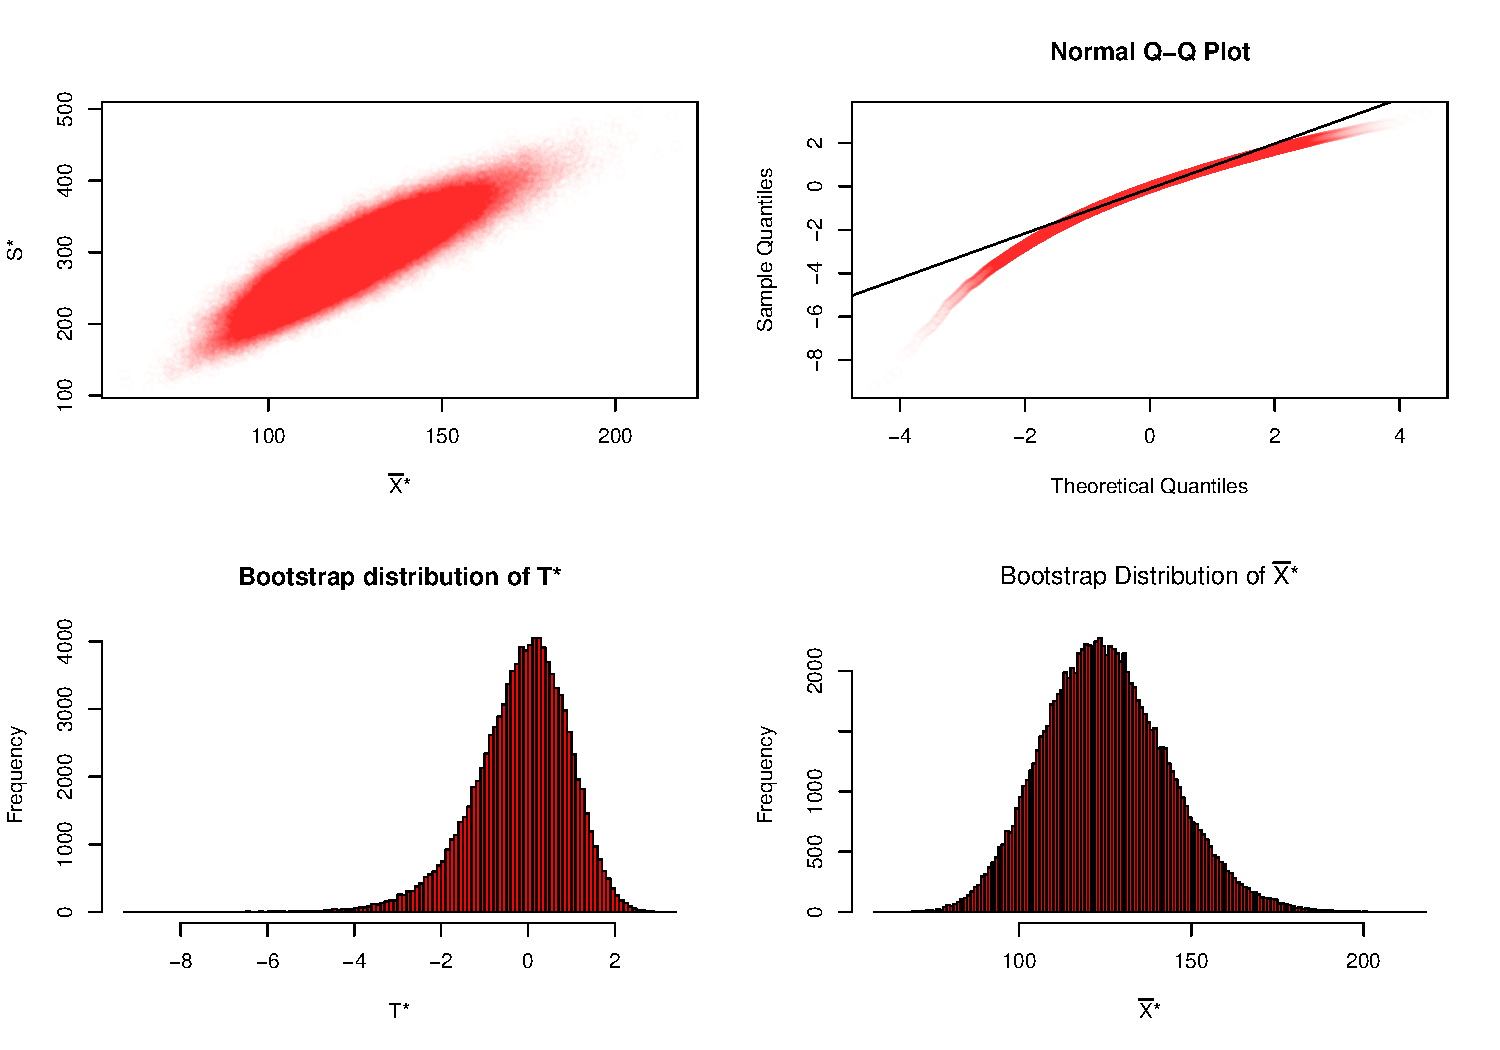
\includegraphics[width=0.7\linewidth,height=0.5\textheight]{Week2_Lect_files/figure-beamer/unnamed-chunk-26-1} \end{center}
\normalsize

\begin{itemize}
\item
  We now have an easier time associating ranges of temperatures to each
  of the bins.
\item
  We can also vary the color of the bars by setting the \texttt{fill}
  argument.
\end{itemize}
\end{frame}

\begin{frame}[fragile]{Histograms via \texttt{geom\_histogram}}
\protect\hypertarget{histograms-via-geom_histogram-3}{}
\tiny

\begin{Shaded}
\begin{Highlighting}[]
\FunctionTok{ggplot}\NormalTok{(}\AttributeTok{data =}\NormalTok{ weather, }\AttributeTok{mapping =} \FunctionTok{aes}\NormalTok{(}\AttributeTok{x =}\NormalTok{ temp)) }\SpecialCharTok{+}
  \FunctionTok{geom\_histogram}\NormalTok{(}\AttributeTok{color =} \StringTok{"black"}\NormalTok{, }\AttributeTok{fill =} \StringTok{"purple"}\NormalTok{) }\SpecialCharTok{+} 
  \FunctionTok{theme\_bw}\NormalTok{()}
\end{Highlighting}
\end{Shaded}

\begin{center}\includegraphics[width=0.7\linewidth,height=0.5\textheight]{Week2_Lect_files/figure-beamer/unnamed-chunk-27-1} \end{center}
\normalsize

\begin{itemize}
\tightlist
\item
  Run \texttt{colors()} to see all 657 possible choice of colors in R!
\item
  Note that in the 50-75\(^{\circ}\)F range there appear to be roughly 8
  bins. Thus each bin has width 25 divided by 8 or 3.125\(^{\circ}\)F.
\end{itemize}
\end{frame}

\begin{frame}[fragile]{Adjusting the bins}
\protect\hypertarget{adjusting-the-bins}{}
\textbf{Method 1}: By adjusting the number of bins via the bins argument
to \texttt{geom\_histogram()}.

\tiny

\begin{Shaded}
\begin{Highlighting}[]
\FunctionTok{ggplot}\NormalTok{(}\AttributeTok{data =}\NormalTok{ weather, }\AttributeTok{mapping =} \FunctionTok{aes}\NormalTok{(}\AttributeTok{x =}\NormalTok{ temp)) }\SpecialCharTok{+}
  \FunctionTok{geom\_histogram}\NormalTok{(}\AttributeTok{bins =} \DecValTok{40}\NormalTok{, }\AttributeTok{color =} \StringTok{"black"}\NormalTok{, }\AttributeTok{fill =} \StringTok{"purple"}\NormalTok{) }\SpecialCharTok{+} 
  \FunctionTok{theme\_bw}\NormalTok{()}
\end{Highlighting}
\end{Shaded}

\begin{center}\includegraphics[width=0.7\linewidth,height=0.5\textheight]{Week2_Lect_files/figure-beamer/unnamed-chunk-28-1} \end{center}
\normalsize
\end{frame}

\begin{frame}[fragile]{Adjusting the bins}
\protect\hypertarget{adjusting-the-bins-1}{}
\textbf{Method 2}: By adjusting the width of the bins via the binwidth
argument to \texttt{geom\_histogram()}

\tiny

\begin{Shaded}
\begin{Highlighting}[]
\FunctionTok{ggplot}\NormalTok{(}\AttributeTok{data =}\NormalTok{ weather, }\AttributeTok{mapping =} \FunctionTok{aes}\NormalTok{(}\AttributeTok{x =}\NormalTok{ temp)) }\SpecialCharTok{+}
  \FunctionTok{geom\_histogram}\NormalTok{(}\AttributeTok{binwidth =} \DecValTok{10}\NormalTok{, }\AttributeTok{color =} \StringTok{"black"}\NormalTok{, }\AttributeTok{fill =} \StringTok{"purple"}\NormalTok{) }\SpecialCharTok{+} 
  \FunctionTok{theme\_bw}\NormalTok{()}
\end{Highlighting}
\end{Shaded}

\begin{center}\includegraphics[width=0.7\linewidth,height=0.5\textheight]{Week2_Lect_files/figure-beamer/unnamed-chunk-29-1} \end{center}
\normalsize
\end{frame}

\begin{frame}{Facets}
\protect\hypertarget{facets}{}
Before continuing with the next of the 5NG, let's briefly introduce a
new concept called \textbf{faceting}.

\begin{itemize}
\item
  Faceting is used when we'd like to split a particular visualization by
  the values of another variable.
\item
  This will create multiple copies of the same type of plot with
  matching x and y axes, but whose content will differ.
\end{itemize}

Example: lets Looking at how the histogram of hourly
\textbf{temperature} recordings at the three NYC airports we saw earlier
differed in each \textbf{month}.
\end{frame}

\begin{frame}[fragile]{Facets}
\protect\hypertarget{facets-1}{}
\tiny

\begin{Shaded}
\begin{Highlighting}[]
\FunctionTok{ggplot}\NormalTok{(}\AttributeTok{data =}\NormalTok{ weather, }\AttributeTok{mapping =} \FunctionTok{aes}\NormalTok{(}\AttributeTok{x =}\NormalTok{ temp)) }\SpecialCharTok{+}
  \FunctionTok{geom\_histogram}\NormalTok{(}\AttributeTok{binwidth =} \DecValTok{5}\NormalTok{, }\AttributeTok{color =} \StringTok{"black"}\NormalTok{, }\AttributeTok{fill =} \StringTok{"lightblue"}\NormalTok{) }\SpecialCharTok{+}
  \FunctionTok{facet\_wrap}\NormalTok{(}\FunctionTok{vars}\NormalTok{(month)) }\SpecialCharTok{+} 
  \FunctionTok{theme\_bw}\NormalTok{()}
\end{Highlighting}
\end{Shaded}

\begin{center}\includegraphics[width=0.7\linewidth,height=0.7\textheight]{Week2_Lect_files/figure-beamer/unnamed-chunk-30-1} \end{center}
\normalsize
\end{frame}

\begin{frame}[fragile]{Facets}
\protect\hypertarget{facets-2}{}
We can also specify the number of rows and columns in the grid by using
the \texttt{nrow} and \texttt{ncol} arguments inside of
\texttt{facet\_wrap()}.

\tiny

\begin{Shaded}
\begin{Highlighting}[]
\FunctionTok{ggplot}\NormalTok{(}\AttributeTok{data =}\NormalTok{ weather, }\AttributeTok{mapping =} \FunctionTok{aes}\NormalTok{(}\AttributeTok{x =}\NormalTok{ temp)) }\SpecialCharTok{+}
  \FunctionTok{geom\_histogram}\NormalTok{(}\AttributeTok{binwidth =} \DecValTok{5}\NormalTok{, }\AttributeTok{color =} \StringTok{"black"}\NormalTok{, }\AttributeTok{fill =} \StringTok{"lightblue"}\NormalTok{) }\SpecialCharTok{+}
  \FunctionTok{facet\_wrap}\NormalTok{(}\FunctionTok{vars}\NormalTok{(month), }\AttributeTok{nrow =} \DecValTok{4}\NormalTok{) }\SpecialCharTok{+}
  \FunctionTok{theme\_bw}\NormalTok{()}
\end{Highlighting}
\end{Shaded}

\begin{center}\includegraphics[width=0.7\linewidth,height=0.6\textheight]{Week2_Lect_files/figure-beamer/unnamed-chunk-31-1} \end{center}
\normalsize
\end{frame}

\begin{frame}{5NG\#4: Boxplots}
\protect\hypertarget{ng4-boxplots}{}
Another type of visualization that can be used to compare the
distribution of a numerical variable split by the values of another
variable is a \textbf{side-by-side boxplot}.

\begin{itemize}
\item
  A \textbf{boxplot} is constructed from the information provided in the
  \textbf{five-number summary} of a numerical variable.
\item
  Let's see an example of a boxplot using hourly temperature recordings
  for the month of November.

  \begin{itemize}
  \tightlist
  \item
    Minimum: 21\(^{\circ}\)F
  \item
    First quartile (25th percentile):36\(^{\circ}\)F
  \item
    Median (second quartile, 50th percentile): 45\(^{\circ}\)F
  \item
    Third quartile (75th percentile): 52\(^{\circ}\)F
  \item
    Maximum: 71\(^{\circ}\)F
  \end{itemize}
\end{itemize}
\end{frame}

\begin{frame}{5NG\#4: Boxplots}
\protect\hypertarget{ng4-boxplots-1}{}
\begin{itemize}
\item
  From the figure below:

  \begin{itemize}
  \tightlist
  \item
    In the leftmost plot let's mark these 5 values with dashed
    horizontal lines on top of the 2141 points(observations).
  \item
    In the middle plot, let's add the boxplot.
  \item
    In the rightmost plot, let's remove the points and the dashed
    horizontal lines for clarity's sake.
  \end{itemize}
\end{itemize}

\tiny

\begin{center}\includegraphics[width=0.7\linewidth,height=0.5\textheight]{Week2_3} \end{center}
\normalsize
\end{frame}

\begin{frame}{5NG\#4: Boxplots}
\protect\hypertarget{ng4-boxplots-2}{}
From the Boxplot:

\begin{itemize}
\item
  25\% of observations were below 36\(^{\circ}\)F.
\item
  25\% of observations were between 36\(^{\circ}\)F and 45\(^{\circ}\)F
  and 50\% of observations were below 45\(^{\circ}\)F.
\item
  25\% of observations were between 45\(^{\circ}\)F and 52\(^{\circ}\)F
  and 75\% of observations were below 52\(^{\circ}\)F.
\item
  25\% of observations were above 52\(^{\circ}\)F.
\item
  The middle 50\% of points lie within the interquartile range (IQR)
  between the first and third quartile. IQR for this example is 52 - 36
  = 16\(^{\circ}\)F.
\end{itemize}
\end{frame}

\begin{frame}{5NG\#4: Boxplots}
\protect\hypertarget{ng4-boxplots-3}{}
From the Boxplot:

\begin{itemize}
\item
  The whiskers stick out from either end of the box all the way to the
  \textbf{minimum}(21\(^{\circ}\)F) and \textbf{maximum} observed
  temperatures (71\(^{\circ}\)F).

  \begin{itemize}
  \tightlist
  \item
    However, the whiskers extend no more than \(1.5 \times\) IQR from
    either end of the box.
  \item
    Any observed values outside this range get marked with points called
    \textbf{outliers}.
  \end{itemize}
\end{itemize}
\end{frame}

\begin{frame}[fragile]{Boxplots via \texttt{geom\_boxplot}: Invalid
specification}
\protect\hypertarget{boxplots-via-geom_boxplot-invalid-specification}{}
\tiny

\begin{Shaded}
\begin{Highlighting}[]
\FunctionTok{ggplot}\NormalTok{(}\AttributeTok{data =}\NormalTok{ weather, }\AttributeTok{mapping =} \FunctionTok{aes}\NormalTok{(}\AttributeTok{x =}\NormalTok{ month, }\AttributeTok{y =}\NormalTok{ temp)) }\SpecialCharTok{+}
  \FunctionTok{geom\_boxplot}\NormalTok{() }\SpecialCharTok{+} 
  \FunctionTok{theme\_bw}\NormalTok{()}
\end{Highlighting}
\end{Shaded}

\begin{center}\includegraphics[width=0.4\linewidth,height=0.5\textheight]{Week2_Lect_files/figure-beamer/unnamed-chunk-33-1} \end{center}
\normalsize

\begin{itemize}
\item
  Observe that this plot does not provide information about temperature
  separated by month.

  \begin{itemize}
  \tightlist
  \item
    Boxplots, require a categorical variable to be mapped to the
    x-position aesthetic. But the \texttt{month} variable is numerical
    variable.
  \end{itemize}
\end{itemize}
\end{frame}

\begin{frame}[fragile]{Boxplots via \texttt{geom\_boxplot}}
\protect\hypertarget{boxplots-via-geom_boxplot}{}
\tiny

\begin{Shaded}
\begin{Highlighting}[]
\FunctionTok{ggplot}\NormalTok{(}\AttributeTok{data =}\NormalTok{ weather, }\AttributeTok{mapping =} \FunctionTok{aes}\NormalTok{(}\AttributeTok{x =} \FunctionTok{factor}\NormalTok{(month), }\AttributeTok{y =}\NormalTok{ temp)) }\SpecialCharTok{+}
  \FunctionTok{geom\_boxplot}\NormalTok{() }\SpecialCharTok{+} 
  \FunctionTok{theme\_bw}\NormalTok{()}
\end{Highlighting}
\end{Shaded}

\begin{center}\includegraphics[width=0.9\linewidth,height=0.5\textheight]{Week2_Lect_files/figure-beamer/unnamed-chunk-34-1} \end{center}
\normalsize

Thus the 12 separate boxplots are shown ``side-by-side.''
\end{frame}

\begin{frame}{5NG\#5: Barplots}
\protect\hypertarget{ng5-barplots}{}
\begin{itemize}
\item
  Both histograms and boxplots are tools to visualize the distribution
  of numerical variables.
\item
  Another commonly desired task is to visualize the distribution of a
  categorical variable.

  \begin{itemize}
  \tightlist
  \item
    we are simply counting different categories within a categorical
    variable, also known as the levels of the categorical variable
  \end{itemize}
\item
  Often the best way to visualize these different counts, also known as
  \textbf{frequencies}, is with \textbf{barplots} (also called
  barcharts).
\end{itemize}
\end{frame}

\begin{frame}[fragile]{5NG\#5: Barplots}
\protect\hypertarget{ng5-barplots-1}{}
\begin{itemize}
\item
  One complication, however, is how your data is represented.

  \begin{itemize}
  \tightlist
  \item
    Is the categorical variable of interest ``pre-counted'' or not?
  \end{itemize}
\item
  For example, run the following code that manually creates two data
  frames representing a collection of fruit: 3 apples and 2 oranges.
\end{itemize}

\tiny

\begin{Shaded}
\begin{Highlighting}[]
\FunctionTok{library}\NormalTok{(dplyr)}
\NormalTok{fruits }\OtherTok{\textless{}{-}} \FunctionTok{tibble}\NormalTok{(}
  \AttributeTok{fruit =} \FunctionTok{c}\NormalTok{(}\StringTok{"apple"}\NormalTok{, }\StringTok{"apple"}\NormalTok{, }\StringTok{"orange"}\NormalTok{, }\StringTok{"apple"}\NormalTok{, }\StringTok{"orange"}\NormalTok{)}
\NormalTok{)}
\NormalTok{fruits\_counted }\OtherTok{\textless{}{-}} \FunctionTok{tibble}\NormalTok{(}
  \AttributeTok{fruit =} \FunctionTok{c}\NormalTok{(}\StringTok{"apple"}\NormalTok{, }\StringTok{"orange"}\NormalTok{),}
  \AttributeTok{number =} \FunctionTok{c}\NormalTok{(}\DecValTok{3}\NormalTok{, }\DecValTok{2}\NormalTok{)}
\NormalTok{)}
\end{Highlighting}
\end{Shaded}

\normalsize
\end{frame}

\begin{frame}[fragile]{5NG\#5: Barplots}
\protect\hypertarget{ng5-barplots-2}{}
\tiny

\begin{Shaded}
\begin{Highlighting}[]
\NormalTok{fruits }
\end{Highlighting}
\end{Shaded}

\begin{verbatim}
# A tibble: 5 x 1
  fruit 
  <chr> 
1 apple 
2 apple 
3 orange
4 apple 
5 orange
\end{verbatim}

\begin{Shaded}
\begin{Highlighting}[]
\NormalTok{fruits\_counted }
\end{Highlighting}
\end{Shaded}

\begin{verbatim}
# A tibble: 2 x 2
  fruit  number
  <chr>   <dbl>
1 apple       3
2 orange      2
\end{verbatim}

\normalsize

Depending on how your categorical data is represented, you'll need to
add a different \texttt{geom}etric layer type to your ggplot() to create
a barplot.
\end{frame}

\begin{frame}[fragile]{Barplots via \texttt{geom\_bar}}
\protect\hypertarget{barplots-via-geom_bar}{}
\tiny

\begin{Shaded}
\begin{Highlighting}[]
\FunctionTok{ggplot}\NormalTok{(}\AttributeTok{data =}\NormalTok{ fruits, }\AttributeTok{mapping =} \FunctionTok{aes}\NormalTok{(}\AttributeTok{x =}\NormalTok{ fruit)) }\SpecialCharTok{+}
  \FunctionTok{geom\_bar}\NormalTok{(}\AttributeTok{fill =} \FunctionTok{c}\NormalTok{(}\StringTok{"red"}\NormalTok{, }\StringTok{"orange"}\NormalTok{)) }\SpecialCharTok{+} 
  \FunctionTok{theme\_bw}\NormalTok{()}
\end{Highlighting}
\end{Shaded}

\begin{center}\includegraphics[width=0.9\linewidth,height=0.5\textheight]{Week2_Lect_files/figure-beamer/unnamed-chunk-37-1} \end{center}
\normalsize

When the categorical variable whose distribution you want to visualize
\textbf{is not pre-counted} in your data frame, we use
\textbf{geom\_bar()}.
\end{frame}

\begin{frame}[fragile]{Barplots via \texttt{geom\_col}}
\protect\hypertarget{barplots-via-geom_col}{}
\tiny

\begin{Shaded}
\begin{Highlighting}[]
\FunctionTok{ggplot}\NormalTok{(}\AttributeTok{data =}\NormalTok{ fruits\_counted, }\AttributeTok{mapping =} \FunctionTok{aes}\NormalTok{(}\AttributeTok{x =}\NormalTok{ fruit, }\AttributeTok{y =}\NormalTok{ number)) }\SpecialCharTok{+}
  \FunctionTok{geom\_col}\NormalTok{(}\AttributeTok{fill =} \FunctionTok{c}\NormalTok{(}\StringTok{"red"}\NormalTok{, }\StringTok{"orange"}\NormalTok{)) }\SpecialCharTok{+} 
  \FunctionTok{theme\_bw}\NormalTok{()}
\end{Highlighting}
\end{Shaded}

\begin{center}\includegraphics[width=0.9\linewidth,height=0.5\textheight]{Week2_Lect_files/figure-beamer/unnamed-chunk-38-1} \end{center}
\normalsize

When the categorical variable whose distribution you want to visualize
\textbf{is pre-counted} in your data frame, we use \textbf{geom\_col()}.
\end{frame}

\begin{frame}[fragile]{Barplots for \texttt{flights} data}
\protect\hypertarget{barplots-for-flights-data}{}
Let's now go back to the \texttt{flights} data frame in the
\texttt{nycflights13} package and visualize the distribution of the
categorical variable \texttt{carrier}.

\begin{itemize}
\tightlist
\item
  Because the \texttt{flights} have \textbf{not been pre-counted} by
  \texttt{carrier}, we use \texttt{geom\_bar()}.
\end{itemize}
\end{frame}

\begin{frame}[fragile]{Barplots for \texttt{flights} data}
\protect\hypertarget{barplots-for-flights-data-1}{}
\tiny

\begin{Shaded}
\begin{Highlighting}[]
\FunctionTok{ggplot}\NormalTok{(}\AttributeTok{data =}\NormalTok{ flights, }\AttributeTok{mapping =} \FunctionTok{aes}\NormalTok{(}\AttributeTok{x =}\NormalTok{ carrier)) }\SpecialCharTok{+}
  \FunctionTok{geom\_bar}\NormalTok{(}\AttributeTok{fill =} \StringTok{"lightblue"}\NormalTok{) }\SpecialCharTok{+} 
  \FunctionTok{theme\_bw}\NormalTok{()}
\end{Highlighting}
\end{Shaded}

\begin{center}\includegraphics[width=0.9\linewidth,height=0.5\textheight]{Week2_Lect_files/figure-beamer/unnamed-chunk-39-1} \end{center}
\normalsize
\end{frame}

\begin{frame}{Pie charts}
\protect\hypertarget{pie-charts}{}
\begin{itemize}
\item
  One of the most common plots used to visualize the distribution of
  categorical data is the \textbf{pie chart}.
\item
  A pie chart presents each category as a slice of a circle so that each
  slice has a size that is proportional to the whole in each category.
\item
  While they may seem harmless enough, pie charts actually present a
  problem in that humans are unable to judge angles well.

  \begin{itemize}
  \tightlist
  \item
    In other words, it is difficult for us to determine the relative
    size of one piece of the pie compared to another.
  \end{itemize}
\item
  This makes barplots preferred in certain situations.
\end{itemize}
\end{frame}

\begin{frame}{Cases Were Barplots are Preferred}
\protect\hypertarget{cases-were-barplots-are-preferred}{}
\begin{center}\includegraphics[width=0.8\linewidth,height=0.7\textheight]{week2_4} \end{center}

It is hard to see the pattern in the pie chart but the bar chart makes
it easier to compare frequencies in groups.
\end{frame}

\begin{frame}[fragile]{Two categorical variables}
\protect\hypertarget{two-categorical-variables}{}
\begin{itemize}
\item
  Barplots are a very common way to visualize the frequency of different
  categories, or levels, of a single categorical variable.
\item
  Another use of barplots is to visualize the joint distribution of
  \textbf{two categorical variables} at the same time.
\end{itemize}

Let's examine the joint distribution of outgoing domestic flights from
NYC by \texttt{carrier} as well as \texttt{origin}.
\end{frame}

\begin{frame}[fragile]{Two categorical variables: Stacked barplot}
\protect\hypertarget{two-categorical-variables-stacked-barplot}{}
\tiny

\begin{Shaded}
\begin{Highlighting}[]
\FunctionTok{ggplot}\NormalTok{(}\AttributeTok{data =}\NormalTok{ flights, }\AttributeTok{mapping =} \FunctionTok{aes}\NormalTok{(}\AttributeTok{x =}\NormalTok{ carrier, }\AttributeTok{fill =}\NormalTok{ origin)) }\SpecialCharTok{+}
  \FunctionTok{geom\_bar}\NormalTok{() }\SpecialCharTok{+} 
  \FunctionTok{theme\_bw}\NormalTok{()}
\end{Highlighting}
\end{Shaded}

\begin{center}\includegraphics[width=0.9\linewidth,height=0.5\textheight]{Week2_Lect_files/figure-beamer/unnamed-chunk-41-1} \end{center}
\normalsize

\begin{itemize}
\tightlist
\item
  This is an example of a \textbf{stacked} barplot.
\item
  The \texttt{fill} aesthetic corresponds to the color used to fill the
  bars
\end{itemize}
\end{frame}

\begin{frame}[fragile]{Two categorical variables: Stacked barplot}
\protect\hypertarget{two-categorical-variables-stacked-barplot-1}{}
\tiny

\begin{Shaded}
\begin{Highlighting}[]
\FunctionTok{ggplot}\NormalTok{(}\AttributeTok{data =}\NormalTok{ flights, }\AttributeTok{mapping =} \FunctionTok{aes}\NormalTok{(}\AttributeTok{x =}\NormalTok{ carrier, }\AttributeTok{color =}\NormalTok{ origin)) }\SpecialCharTok{+}
  \FunctionTok{geom\_bar}\NormalTok{() }\SpecialCharTok{+} 
  \FunctionTok{theme\_bw}\NormalTok{()}
\end{Highlighting}
\end{Shaded}

\begin{center}\includegraphics[width=0.9\linewidth,height=0.5\textheight]{Week2_Lect_files/figure-beamer/unnamed-chunk-42-1} \end{center}
\normalsize

\begin{itemize}
\tightlist
\item
  The \texttt{color} aesthetic corresponds to the color of the outline
  of the bars.
\end{itemize}
\end{frame}

\begin{frame}[fragile]{Two categorical variables: side-by-side barplots}
\protect\hypertarget{two-categorical-variables-side-by-side-barplots}{}
While simple to make, in certain aspects it is not ideal.

\begin{itemize}
\item
  For example, it is difficult to compare the heights of the different
  colors between the bars, corresponding to comparing the number of
  flights from each origin airport between the carriers.
\item
  An alternative to stacked barplots are \textbf{side-by-side barplots},
  also known as \textbf{dodged barplots}.
\item
  The code to create a side-by-side barplot is identical to the code to
  create a stacked barplot, but with a \texttt{position\ =\ "dodge"}
  argument added to \texttt{geom\_bar()}.

  \begin{itemize}
  \tightlist
  \item
    we are overriding the default barplot type, which is a stacked
    barplot.
  \end{itemize}
\end{itemize}
\end{frame}

\begin{frame}[fragile]{Two categorical variables: side-by-side barplots}
\protect\hypertarget{two-categorical-variables-side-by-side-barplots-1}{}
\tiny

\begin{Shaded}
\begin{Highlighting}[]
\FunctionTok{ggplot}\NormalTok{(}\AttributeTok{data =}\NormalTok{ flights, }\AttributeTok{mapping =} \FunctionTok{aes}\NormalTok{(}\AttributeTok{x =}\NormalTok{ carrier, }\AttributeTok{fill =}\NormalTok{ origin)) }\SpecialCharTok{+}
  \FunctionTok{geom\_bar}\NormalTok{(}\AttributeTok{position =} \StringTok{"dodge"}\NormalTok{) }\SpecialCharTok{+} 
  \FunctionTok{theme\_bw}\NormalTok{()}
\end{Highlighting}
\end{Shaded}

\begin{center}\includegraphics[width=0.9\linewidth,height=0.5\textheight]{Week2_Lect_files/figure-beamer/unnamed-chunk-43-1} \end{center}
\normalsize

\begin{itemize}
\tightlist
\item
  Note the width of the bars for AS, F9, FL, HA and YV is different than
  the others
\item
  To be the same size in terms of width as the other bars we use a more
  robust \texttt{position\_dodge()} function.
\end{itemize}
\end{frame}

\begin{frame}[fragile]{Two categorical variables: side-by-side barplots}
\protect\hypertarget{two-categorical-variables-side-by-side-barplots-2}{}
\tiny

\begin{Shaded}
\begin{Highlighting}[]
\FunctionTok{ggplot}\NormalTok{(}\AttributeTok{data =}\NormalTok{ flights, }\AttributeTok{mapping =} \FunctionTok{aes}\NormalTok{(}\AttributeTok{x =}\NormalTok{ carrier, }\AttributeTok{fill =}\NormalTok{ origin)) }\SpecialCharTok{+}
  \FunctionTok{geom\_bar}\NormalTok{(}\AttributeTok{position =} \FunctionTok{position\_dodge}\NormalTok{(}\AttributeTok{preserve =} \StringTok{"single"}\NormalTok{)) }\SpecialCharTok{+} 
  \FunctionTok{theme\_bw}\NormalTok{()}
\end{Highlighting}
\end{Shaded}

\begin{center}\includegraphics[width=0.9\linewidth,height=0.5\textheight]{Week2_Lect_files/figure-beamer/unnamed-chunk-44-1} \end{center}
\normalsize
\end{frame}

\begin{frame}[fragile]{Two categorical variables: side-by-side barplots}
\protect\hypertarget{two-categorical-variables-side-by-side-barplots-3}{}
Change order:

\tiny

\begin{Shaded}
\begin{Highlighting}[]
\NormalTok{flights1 }\OtherTok{\textless{}{-}}\NormalTok{ flights}
\NormalTok{flights1}\SpecialCharTok{$}\NormalTok{origin1 }\OtherTok{\textless{}{-}} \FunctionTok{factor}\NormalTok{(flights1}\SpecialCharTok{$}\NormalTok{origin, }\AttributeTok{ordered =} \ConstantTok{TRUE}\NormalTok{,}
\AttributeTok{levels =} \FunctionTok{c}\NormalTok{(}\StringTok{"JFK"}\NormalTok{, }\StringTok{"EWR"}\NormalTok{, }\StringTok{"LGA"}\NormalTok{))}

\FunctionTok{ggplot}\NormalTok{(}\AttributeTok{data =}\NormalTok{ flights1, }\AttributeTok{mapping =} \FunctionTok{aes}\NormalTok{(}\AttributeTok{x =}\NormalTok{ carrier, }\AttributeTok{fill =}\NormalTok{ origin1)) }\SpecialCharTok{+}
  \FunctionTok{geom\_bar}\NormalTok{(}\AttributeTok{position =} \FunctionTok{position\_dodge}\NormalTok{(}\AttributeTok{preserve =} \StringTok{"single"}\NormalTok{)) }\SpecialCharTok{+} 
  \FunctionTok{theme\_bw}\NormalTok{()}
\end{Highlighting}
\end{Shaded}

\begin{center}\includegraphics[width=0.9\linewidth,height=0.5\textheight]{Week2_Lect_files/figure-beamer/unnamed-chunk-45-1} \end{center}
\normalsize
\end{frame}

\begin{frame}[fragile]{Two categorical variables: faceted barplot}
\protect\hypertarget{two-categorical-variables-faceted-barplot}{}
\tiny

\begin{Shaded}
\begin{Highlighting}[]
\FunctionTok{ggplot}\NormalTok{(}\AttributeTok{data =}\NormalTok{ flights, }\AttributeTok{mapping =} \FunctionTok{aes}\NormalTok{(}\AttributeTok{x =}\NormalTok{ carrier)) }\SpecialCharTok{+}
  \FunctionTok{geom\_bar}\NormalTok{(}\AttributeTok{fill =} \StringTok{"pink"}\NormalTok{) }\SpecialCharTok{+}
  \FunctionTok{facet\_wrap}\NormalTok{(}\FunctionTok{vars}\NormalTok{(origin), }\AttributeTok{ncol =} \DecValTok{1}\NormalTok{) }\SpecialCharTok{+} 
  \FunctionTok{theme\_bw}\NormalTok{()}
\end{Highlighting}
\end{Shaded}

\begin{center}\includegraphics[width=0.7\linewidth,height=0.6\textheight]{Week2_Lect_files/figure-beamer/unnamed-chunk-46-1} \end{center}
\normalsize
\end{frame}

\begin{frame}{Summary table}
\protect\hypertarget{summary-table}{}
\begin{figure}[h]

{\centering \includegraphics[width=0.8\linewidth,height=0.7\textheight]{week2_5} 

}

\caption{Summary of Five Named Graphs}\label{fig:5NG}
\end{figure}
\end{frame}

\end{document}
